\documentclass[a4paper,12pt]{article}

% ---------------- Encoding & Language ----------------
\usepackage[utf8]{inputenc}
\usepackage[T5]{fontenc} % better for Vietnamese diacritics
\usepackage[english,vietnamese]{babel}

% ---------------- Packages ----------------
\usepackage{amsmath,amssymb}
\usepackage{array}
\usepackage{textcomp}
\usepackage{xcolor}
\usepackage{graphicx}
\usepackage{geometry}
\usepackage{float}
\usepackage{mdframed}
\usepackage{nopageno}
\usepackage{fancyhdr}
\usepackage{ulem}
\usepackage{tcolorbox}
\usepackage{tocloft}
\usepackage{hyperref}
\usepackage{subcaption}
\usepackage{listings}
\usepackage{longtable}
\usepackage{booktabs}
\usepackage{tabularx}
\usepackage{adjustbox}

% ---------------- Page setup ----------------
\geometry{a4paper, margin=0.75in}
\setlength{\parindent}{0pt} % remove paragraph indentation so lines start flush left

\mdfdefinestyle{MyFrame}{%
    linecolor=blue,
    outerlinewidth=2pt,
    roundcorner=0pt,
    innertopmargin=10pt,
    innerbottommargin=10pt,
    innerrightmargin=10pt,
    innerleftmargin=10pt,
    backgroundcolor=white
}

% ---------------- Colors for listings ----------------
\definecolor{comment}{RGB}{0,128,0}   % green for comments
\definecolor{kwpink}{RGB}{255,20,147} % pink for keywords
\definecolor{numblue}{RGB}{0,0,200}   % blue for numeric literals
\definecolor{string}{RGB}{163,21,21}  % string color (dark red)
\definecolor{framegray}{RGB}{200,200,200}

% ---------------- Listing configuration ----------------
% ---------------- Listing configuration ----------------
\lstset{
    language=C,                       % use C syntax highlighting
    basicstyle=\ttfamily\small,
    keywordstyle=\color{kwpink}\bfseries, % pink for keywords
    commentstyle=\color{comment}\itshape, % green comments
    stringstyle=\color{string},        % dark red strings
    numbers=left,
    numberstyle=\tiny\color{gray},
    stepnumber=1,
    numbersep=6pt,
    backgroundcolor=\color{white},
    frame=single,
    rulecolor=\color{framegray},
    breaklines=true,
    tabsize=4,
    showspaces=false,
    showstringspaces=false,
    alsoletter={_},
    morekeywords={if,else,while,for,switch,case,return}, % only control-flow pink
    deletekeywords={HAL_Delay}, % make sure HAL_Delay is not colored as keyword
    literate=%
     *{0}{{{\color{numblue}0}}}1
      {1}{{{\color{numblue}1}}}1
      {2}{{{\color{numblue}2}}}1
      {3}{{{\color{numblue}3}}}1
      {4}{{{\color{numblue}4}}}1
      {5}{{{\color{numblue}5}}}1
      {6}{{{\color{numblue}6}}}1
      {7}{{{\color{numblue}7}}}1
      {8}{{{\color{numblue}8}}}1
      {9}{{{\color{numblue}9}}}1
      {.}{{{\color{numblue}.}}}1
}

% ---------------- Header / Footer ----------------
\pagestyle{fancy}
\fancyhf{}
\fancyhead[L]{\small Ho Chi Minh City University of Technology \\ Faculty of Computer Science and Engineering}
\fancyhead[R]{
\includegraphics[height=20pt]{bk_logo.png}}
\fancyfoot[C]{\thepage}
\renewcommand{\headrulewidth}{1.5pt}
\renewcommand{\footrulewidth}{1.5pt}

% ---------------- Document ----------------
\begin{document}
\selectlanguage{vietnamese}

\begin{mdframed}[style=MyFrame]
\thispagestyle{empty}
\begin{center}
    \vspace*{0.5cm}
    {\large \textbf{TRƯỜNG ĐẠI HỌC BÁCH KHOA – TP. HỒ CHÍ MINH}}\\[0.2cm]
    {\large \textbf{KHOA KHOA HỌC VÀ KỸ THUẬT MÁY TÍNH}}\\[0.5cm]
    \textbf{*******************}\\[1cm]

    
\includegraphics[width=0.3\textwidth]{bk_logo.png}\\[2cm]

    {\LARGE \textbf{Lab 2}}\\[0.5cm]
    {\LARGE \textbf{Timer Interrupt and LED Scanning}}\\[0.5cm]
    {\LARGE \textcolor{blue}{Microcontroller - Microprocessor (Lab)}}\\[0.5cm]
    {\LARGE \textbf{COURSE ID: CO3010 - HK251}}\\[0.5cm]
    \textbf{\large Name: Trương Gia Hy   -   Student ID: 2352458}\\[0.5cm]
    \textbf{\large Supervising Lecturer: Dr. VÕ TUẤN BÌNH}\\[7.0cm]

    {\large TP. Hồ Chí Minh – 2024}
\end{center}
\end{mdframed}

\newpage
\section{Exercise}
The GitHub link for the lab files:
\textcolor{blue}{\url{https://github.com/hygameo/VXL-VDK_2352458}}
\subsection{Exercise 1}
\subsubsection{Report 1: Capture your schematic from Proteus and show in the report.}
\label{ex1r1}
\begin{figure}[H]
    \centering
    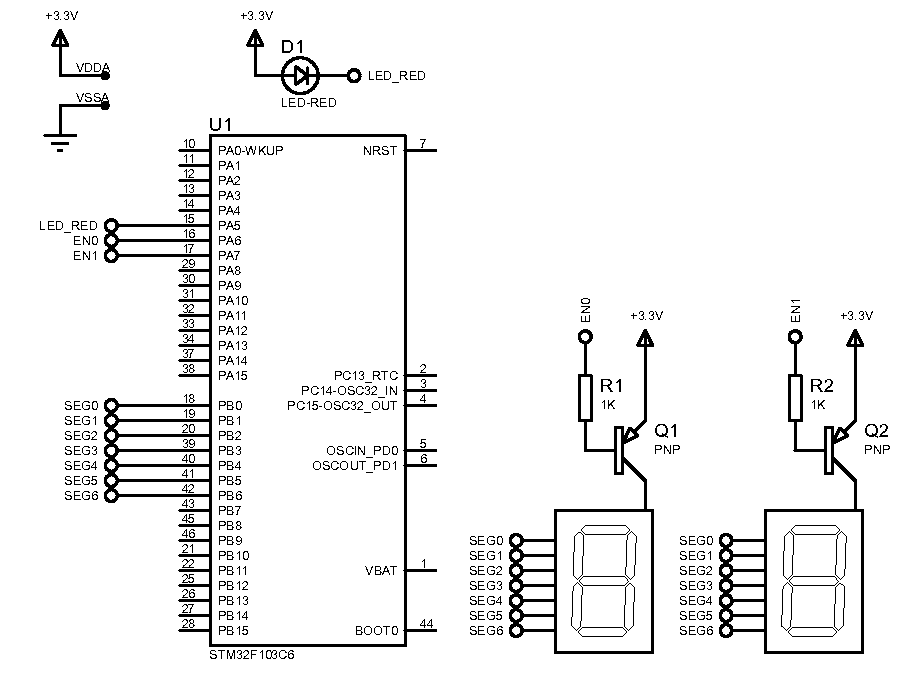
\includegraphics[width=0.95\linewidth]{Attachments/1.1.1.PDF}
\end{figure}
\subsubsection{Report 2: Present your source code.}
\begin{lstlisting}
uint8_t segmentMap[10] = {
	0b1111110, 0b0110000,
	0b1101101, 0b1111001,
	0b0110011, 0b1011011,
	0b1011111, 0b1110000,
	0b1111111, 0b1111011
};

uint8_t SegPin[7] = {
	SEG_A_Pin, SEG_B_Pin,
	SEG_C_Pin, SEG_D_Pin,
	SEG_E_Pin, SEG_F_Pin,
	SEG_G_Pin
};

int counter = 0;
int DisplayNum = 0;

void display7SEG(int num) {
	uint8_t bitmask = segmentMap[num];
	
	for(int i = 0; i < 7; i++) HAL_GPIO_WritePin(GPIOB, SegPin[i], (bitmask & (1 << (6 - i))) ? RESET : SET);
}

void HAL_TIM_PeriodElapsedCallback ( TIM_HandleTypeDef * htim )
{
	counter++;
	if(counter >= 50){
		counter = 0;
		
		HAL_GPIO_WritePin(GPIOA, EN0_Pin | EN1_Pin, GPIO_PIN_SET);
		
		if(DisplayNum == 0){
			HAL_GPIO_WritePin(GPIOA, EN0_Pin, GPIO_PIN_RESET);
			display7SEG(1);
		}
		if(DisplayNum == 1){
			HAL_GPIO_TogglePin(GPIOA, LED_RED_Pin);
			HAL_GPIO_WritePin(GPIOA, EN1_Pin, GPIO_PIN_RESET);
			display7SEG(2);
		}
		
		DisplayNum = (DisplayNum + 1) % 2;
	}
}
\end{lstlisting}
\subsubsection{Question: What is the frequency of the scanning process?}

The frequency of the scanning process is 1 Hz, as the switching time between the two seven-segment displays is half a second (0.5 seconds), resulting in one complete cycle (switching from the first to the second and back) every 1 second.
\newpage
\subsection{Exercise 2}
\subsubsection{Report 1: Capture your schematic from Proteus and show in the report.}
\label{ex2r1}
\begin{figure}[H]
	\centering
	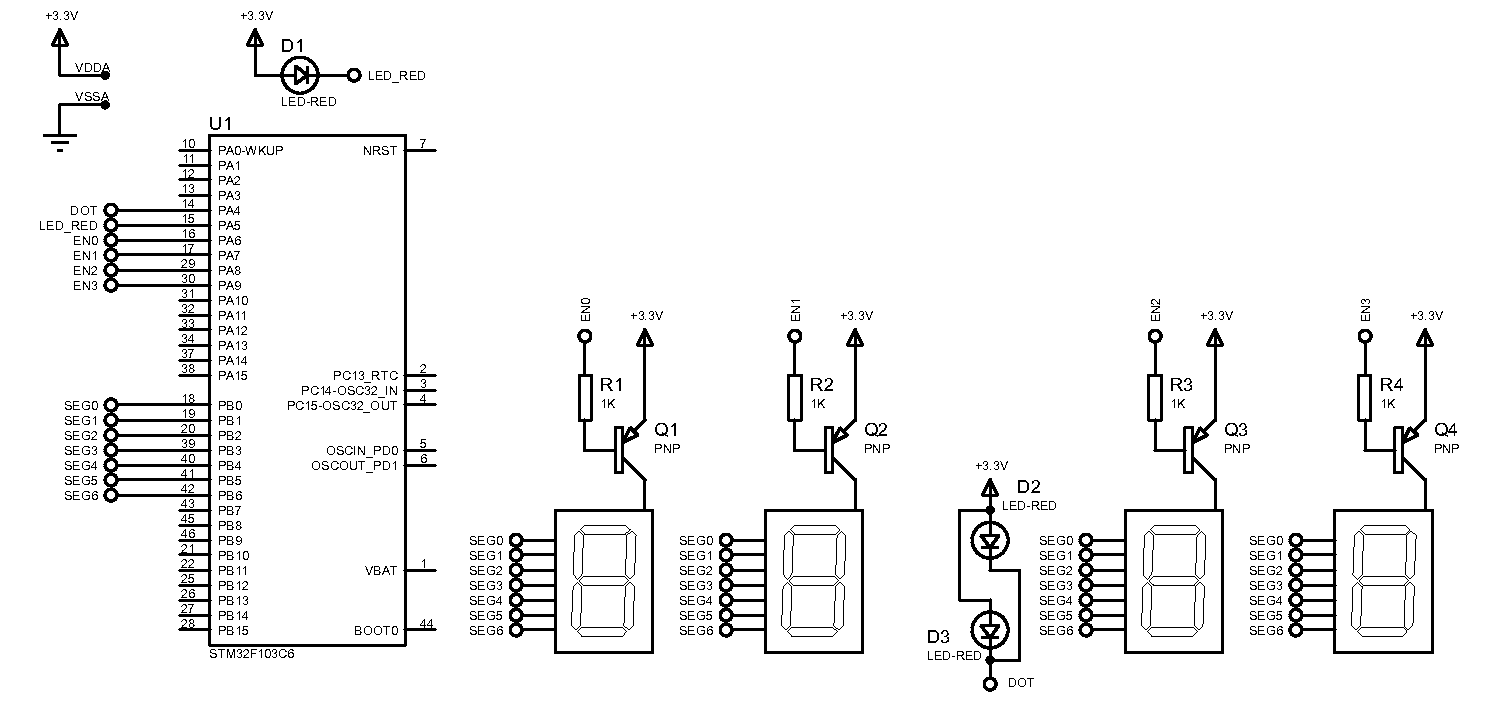
\includegraphics[width=0.95\linewidth]{Attachments/1.2.1.PDF}
\end{figure}
\subsubsection{Report 2: Present your source code.}
\begin{lstlisting}
void HAL_TIM_PeriodElapsedCallback ( TIM_HandleTypeDef * htim )
{
	counter++;
	if(counter >= 50){
		counter = 0;
		
		HAL_GPIO_WritePin(GPIOA, EN0_Pin | EN1_Pin | EN2_Pin | EN3_Pin, GPIO_PIN_SET);
		
		if(DisplayNum == 0){
			HAL_GPIO_WritePin(GPIOA, EN0_Pin, GPIO_PIN_RESET);
			display7SEG(1);
		}
		if(DisplayNum == 1){
			HAL_GPIO_TogglePin(GPIOA, LED_RED_Pin | DOT_Pin);
			HAL_GPIO_WritePin(GPIOA, EN1_Pin, GPIO_PIN_RESET);
			display7SEG(2);
		}
		if(DisplayNum == 2){
			HAL_GPIO_WritePin(GPIOA, EN2_Pin, GPIO_PIN_RESET);
			display7SEG(3);
		}
		if(DisplayNum == 3){
			HAL_GPIO_TogglePin(GPIOA, LED_RED_Pin | DOT_Pin);
			HAL_GPIO_WritePin(GPIOA, EN3_Pin, GPIO_PIN_RESET);
			display7SEG(0);
		}
		DisplayNum = (DisplayNum + 1) % 4;
	}
}
\end{lstlisting}
\subsubsection{Question: What is the frequency of the scanning process?}

The frequency of the scanning process is 0.5 Hz. This is because each seven-segment LED is displayed for 500ms (0.5 seconds), and the system cycles through all 4 LEDs, completing one full scan every 2 seconds (4 x 0.5s = 2s). The frequency is calculated as $ \frac{1}{2} $ Hz.
\subsection{Exercise 3}
\subsubsection{Report 1: Present the source code of the update7SEG function.}
\begin{lstlisting}
void update7SEG(int index){
	HAL_GPIO_WritePin(GPIOA, EN0_Pin | EN1_Pin | EN2_Pin | EN3_Pin, GPIO_PIN_SET);
	
	switch (index){
		case 0:
		HAL_GPIO_WritePin(GPIOA, GPIO_PIN_6, GPIO_PIN_RESET);
		display7SEG(led_buffer[0]);
		break;
		case 1:
		HAL_GPIO_WritePin(GPIOA, GPIO_PIN_7, GPIO_PIN_RESET);
		display7SEG(led_buffer[1]);
		break;
		case 2:
		HAL_GPIO_WritePin(GPIOA, GPIO_PIN_8, GPIO_PIN_RESET);
		display7SEG(led_buffer[2]);
		break;
		case 3:
		HAL_GPIO_WritePin(GPIOA, GPIO_PIN_9, GPIO_PIN_RESET);
		display7SEG(led_buffer[3]);
		break;
		default:
		break;
	}
}
\end{lstlisting}
\subsubsection{Report 2: Present the source code.}
\begin{lstlisting}
void HAL_TIM_PeriodElapsedCallback ( TIM_HandleTypeDef * htim )
{
	counter++;
	if(counter0 >= 50){
		counter = 0;
		
		if(index_led == 1 || index_led == 3) HAL_GPIO_TogglePin(GPIOA, LED_RED_Pin | DOT_Pin);
		update7SEG(index_led++);
		if(index_led >= 4) index_led = 0;
	}
}
\end{lstlisting}
\subsection{Exercise 4}
\subsubsection{Report 1: Present the source code.}
\begin{lstlisting}
void HAL_TIM_PeriodElapsedCallback ( TIM_HandleTypeDef * htim )
{
	counter++;
	if(counter >= 25){
		counter = 0;
		
		if(index_led == 3) HAL_GPIO_TogglePin(GPIOA, LED_RED_Pin | DOT_Pin);
		update7SEG(index_led++);
		if(index_led >= 4) index_led = 0;
	}
}
\end{lstlisting}
\subsection{Exercise 5}
\subsubsection{Report 1: Present the source code in the updateClockBuffer function.}
\begin{lstlisting}
void updateClockBuffer() {
	led_buffer[0] = hour / 10;
	led_buffer[1] = hour % 10;
	led_buffer[2] = minute / 10;
	led_buffer[3] = minute % 10;
}
\end{lstlisting}
\newpage
\subsection{Exercise 6}
\subsubsection{Report 1: if in line 1 of the code above is miss, what happens after that and why?}
\begin{verbatim}
	    If the line setTimer0(1000) is removed before the while (1) loop, the global 
	variable timer0_counter will remain at its default value of 0. As a result, when 
	timer_run() is called, the condition if (timer0_counter > 0) will be false, and 
	timer0_counter will not decrement. Consequently, timer0_flag will stay at 0 and 
	never be set to 1. In the while (1) loop, the condition if (timer0_flag == 1) will 
	never be true, so HAL_GPIO_TogglePin(GPIOA, LED_RED_Pin) and setTimer0(2000) will 
	not execute. 
	    Since LED_RED is connected with one pin to 3.3V and the signal pin to PA5,
	and PA5 remains in its initial state (GPIO_PIN_RESET), the LED will turn on 
	continuously. This happens because the timer mechanism does not start without 
	initializing timer0_counter with a positive value.
\end{verbatim}
\subsubsection{Report 2: if in line 1 of the code above is changed to setTimer0(1), what happens after
	that and why?}
\begin{verbatim}
	    If setTimer0(1000) is changed to setTimer0(1), the LED_RED will not toggle at 
	all, and the program will remain in an idle state within the while (1) loop. This 
	occurs because timer0_counter is set to 0 due to integer division, preventing the 
	timer_run function from decrementing it or setting timer0_flag to 1, thus blocking 
	the intended logic from executing. The LED will stayed active like Report 1.
\end{verbatim}
\subsubsection{Report 3: If in line 1 of the code above is changed to setTimer0(10), what is changed compared to 2 first questions and why?}
\begin{verbatim}
	    Compared to first question (setTimer0(1000)): The initial delay changes from 
 	1 second to 10ms, making the first LED toggle occur much sooner, though subsequent 
	toggles remain on a 2-second interval.
	    Compared to second question(setTimer0(1)): The system now functions instead 
	of being stuck, because timer0_counter is 1 rather than 0, allowing the timer to run.
	    Reason: The behavior depends on the value of timer0_counter set by duration / 
	TIMER_CYCLE. A value of 1 (from setTimer0(10)) provides a minimal but 
	functional delay, while 100 (from setTimer0(1000)) gives a 1-second delay, and 
	0 (from setTimer0(1)) disables the timer.
\end{verbatim}
\newpage
\subsection{Exercise 7}
\subsubsection{Report 1: Present the source code of this function.}
\begin{lstlisting}
void clearAllClock(void) {
	for (int i = 0; i < 12; i++) HAL_GPIO_WritePin(GPIOA, ACLOCK_Pins[i], GPIO_PIN_RESET);
}
\end{lstlisting}
\subsection{Exercise 8}
\subsubsection{Report 1: Present your source code in the the main function. In the case more extra functions are used (e.g. the second software timer), present them in the report as well.}
\begin{lstlisting}
int timer0_counter = 0;
int timer0_flag = 0;
int timer1_counter = 0;
int timer1_flag = 0;
int TIMER_CYCLE = 10;

void setTimer0 ( int duration ){
	timer0_counter = duration / TIMER_CYCLE ;
	timer0_flag = 0;
}

void setTimer1(int duration) {
	timer1_counter = duration / TIMER_CYCLE;
	timer1_flag = 0;
}

void timer_run() {
	if (timer0_counter > 0) {
		timer0_counter--;
		if (timer0_counter == 0) timer0_flag = 1;
	}
	if (timer1_counter > 0) {
		timer1_counter--;
		if (timer1_counter == 0) timer1_flag = 1;
	}
}

int main(void)
{
	setTimer0(1000) ;
	setTimer1(250) ;
	while (1)
	{
		if(timer0_flag == 1){
			if(counter >= 2){
				HAL_GPIO_TogglePin(GPIOA, LED_RED_Pin);
				counter = 0;
			}
			counter++;
			updateClockBuffer();
			second ++;
			
			if ( second >= 60) {
				second = 0;
				minute++;
			}
			if( minute >= 60) {
				minute = 0;
				hour++;
			}
			if( hour >= 24){
				hour = 0;
			}
			
			HAL_GPIO_TogglePin(GPIOA, DOT_Pin);
			setTimer0(1000) ;
			
		}
		if(timer1_flag == 1){
			update7SEG(index_led++);
			if(index_led >= 4) index_led = 0;
			setTimer1(250) ;
		}
	}
}
\end{lstlisting}
\newpage
\subsection{Exercise 9}
\subsubsection{Report 1: Present the schematic of your system by capturing the screen in Proteus.}
\label{ex3r1}
\begin{figure}[H]
	\centering
	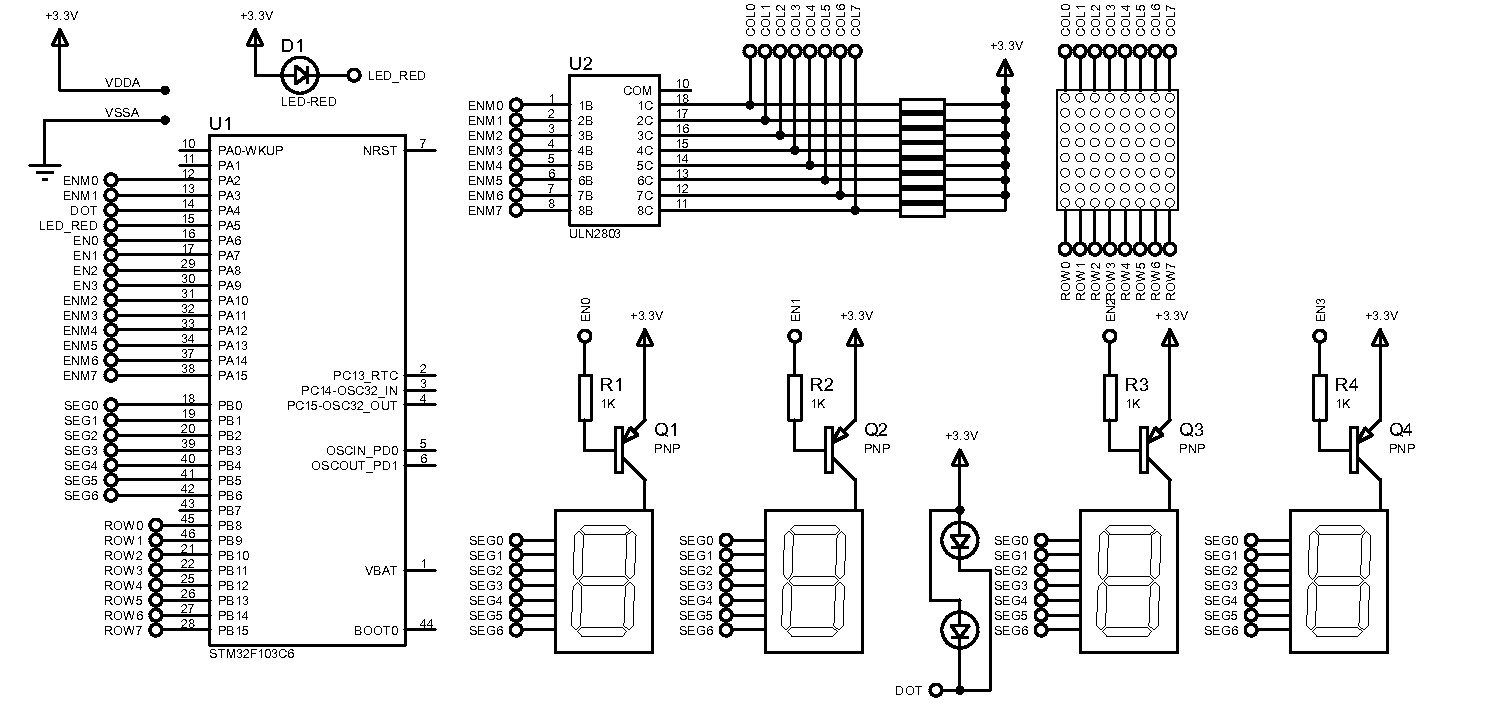
\includegraphics[width=0.95\linewidth]{Attachments/1.9.1.PDF}
\end{figure}
\subsubsection{Report 2: Display character "A".}
\begin{lstlisting}
const int MAX_LED_MATRIX = 8;
int index_led_matrix = 0;
uint8_t matrix_buffer [8] = {0x00, 0x00, 0x7C, 0x12, 0x12, 0x7C, 0x00, 0x00};

void updateLEDMatrix (int index){
	HAL_GPIO_WritePin(GPIOA, ENM0_Pin | ENM1_Pin | ENM2_Pin | ENM3_Pin | ENM4_Pin | ENM5_Pin | ENM6_Pin | ENM7_Pin, GPIO_PIN_SET);
	
	HAL_GPIO_WritePin(GPIOA, ENMPin[index], GPIO_PIN_RESET);
	
	for(int i = 0; i < 8; i++) HAL_GPIO_WritePin(GPIOB, ROWPin[i], (matrix_buffer[index] & (1 << i)) ? GPIO_PIN_RESET : GPIO_PIN_SET);
}

int main(void)
{
	setTimer0(1000) ;
	setTimer1(250) ;
	setTimer2(10) ;
	while (1)
	{
		if(timer0_flag == 1){
			if(counter >= 2){
				HAL_GPIO_TogglePin(GPIOA, LED_RED_Pin);
				counter = 0;
			}
			counter++;
			updateClockBuffer();
			second ++;
			
			if ( second >= 60) {
				second = 0;
				minute++;
			}
			if( minute >= 60) {
				minute = 0;
				hour++;
			}
			if( hour >= 24){
				hour = 0;
			}
			
			HAL_GPIO_TogglePin(GPIOA, DOT_Pin);
			setTimer0(1000) ;
			
		}
		if(timer1_flag == 1){
			update7SEG(index_led++);
			if(index_led >= 4) index_led = 0;
			setTimer1(250) ;
		}
		if(timer2_flag == 1){
			updateLEDMatrix(index_led_matrix);
			index_led_matrix = (index_led_matrix + 1) % MAX_LED_MATRIX;
			setTimer2(10) ;
		}
	}
}
\end{lstlisting}
\newpage
\subsection{Exercise 10}
\subsubsection{Report 1: Present your source code in the report.}
\begin{lstlisting}
uint8_t segmentMap[10] = {
	0b1111110, 0b0110000,
	0b1101101, 0b1111001,
	0b0110011, 0b1011011,
	0b1011111, 0b1110000,
	0b1111111, 0b1111011
};

uint8_t SegPin[7] = {
	SEG_A_Pin, SEG_B_Pin,
	SEG_C_Pin, SEG_D_Pin,
	SEG_E_Pin, SEG_F_Pin,
	SEG_G_Pin
};

uint16_t ENMPin[8] = {
	ENM0_Pin, ENM1_Pin,
	ENM2_Pin, ENM3_Pin,
	ENM4_Pin, ENM5_Pin,
	ENM6_Pin, ENM7_Pin
};

uint16_t ROWPin[8] = {
	ROW0_Pin, ROW1_Pin,
	ROW2_Pin, ROW3_Pin,
	ROW4_Pin, ROW5_Pin,
	ROW6_Pin, ROW7_Pin
};

int timer0_counter = 0;
int timer0_flag = 0;
int timer1_counter = 0;
int timer1_flag = 0;
int timer2_counter = 0;
int timer2_flag = 0;
int TIMER_CYCLE = 10;

const int MAX_LED = 4;
int index_led = 0;
int led_buffer [4] = {1, 2, 3, 4};
int hour = 15, minute = 8, second = 50;

const int MAX_LED_MATRIX = 8;
int index_led_matrix = 0;
uint8_t matrix_buffer [8] = {0x00, 0x00, 0x7C, 0x12, 0x12, 0x7C, 0x00, 0x00};

int counter = 0;

void setTimer0 ( int duration ){
	timer0_counter = duration / TIMER_CYCLE ;
	timer0_flag = 0;
}

void setTimer1(int duration) {
	timer1_counter = duration / TIMER_CYCLE;
	timer1_flag = 0;
}
void setTimer2(int duration) {
	timer2_counter = duration / TIMER_CYCLE;
	timer2_flag = 0;
}

void timer_run() {
	if (timer0_counter > 0) {
		timer0_counter--;
		if (timer0_counter == 0) timer0_flag = 1;
	}
	if (timer1_counter > 0) {
		timer1_counter--;
		if (timer1_counter == 0) timer1_flag = 1;
	}
	if (timer2_counter > 0) {
		timer2_counter--;
		if (timer2_counter == 0) timer2_flag = 1;
	}
}

void display7SEG(int num) {
	for(int i = 0; i < 7; i++) HAL_GPIO_WritePin(GPIOB, SegPin[i], (segmentMap[num] & (1 << (6 - i))) ? RESET : SET);
}

void update7SEG(int index){
	HAL_GPIO_WritePin(GPIOA, EN0_Pin | EN1_Pin | EN2_Pin | EN3_Pin, GPIO_PIN_SET);
	
	switch (index){
		case 0:
		HAL_GPIO_WritePin(GPIOA, EN0_Pin, GPIO_PIN_RESET);
		display7SEG(led_buffer[0]);
		break;
		case 1:
		HAL_GPIO_WritePin(GPIOA, EN1_Pin, GPIO_PIN_RESET);
		display7SEG(led_buffer[1]);
		break;
		case 2:
		HAL_GPIO_WritePin(GPIOA, EN2_Pin, GPIO_PIN_RESET);
		display7SEG(led_buffer[2]);
		break;
		case 3:
		HAL_GPIO_WritePin(GPIOA, EN3_Pin, GPIO_PIN_RESET);
		display7SEG(led_buffer[3]);
		break;
		default:
		break;
	}
}

void updateClockBuffer() {
	led_buffer[0] = hour / 10;
	led_buffer[1] = hour % 10;
	led_buffer[2] = minute / 10;
	led_buffer[3] = minute % 10;
}

void updateLEDMatrix (int index){
	HAL_GPIO_WritePin(GPIOA, ENM0_Pin | ENM1_Pin | ENM2_Pin | ENM3_Pin | ENM4_Pin | ENM5_Pin | ENM6_Pin | ENM7_Pin, GPIO_PIN_SET);
	
	HAL_GPIO_WritePin(GPIOA, ENMPin[index], GPIO_PIN_RESET);
	
	for(int i = 0; i < 8; i++) HAL_GPIO_WritePin(GPIOB, ROWPin[i], (matrix_buffer[index] & (1 << i)) ? GPIO_PIN_RESET : GPIO_PIN_SET);
}

void shiftArray(uint8_t *array, int size) {
	uint8_t temp = array[0];
	for (int i = 0; i < size - 1; i++) array[i] = array[i + 1];
	array[size - 1] = temp;
}

int main(void)
{
	setTimer0(1000) ;
	setTimer1(250) ;
	setTimer2(20) ;
	while (1)
	{
		/* USER CODE END WHILE */
		
		/* USER CODE BEGIN 3 */
		if(timer0_flag == 1){
			if(counter >= 2){
				HAL_GPIO_TogglePin(GPIOA, LED_RED_Pin);
				counter = 0;
			}
			counter++;
			updateClockBuffer();
			second ++;
			
			if ( second >= 60) {
				second = 0;
				minute++;
			}
			if( minute >= 60) {
				minute = 0;
				hour++;
			}
			if( hour >= 24){
				hour = 0;
			}
			
			HAL_GPIO_TogglePin(GPIOA, DOT_Pin);
			setTimer0(1000) ;
			
		}
		if(timer1_flag == 1){
			update7SEG(index_led++);
			if(index_led >= 4) index_led = 0;
			shiftArray(matrix_buffer, MAX_LED_MATRIX);
			setTimer1(250) ;
		}
		if(timer2_flag == 1){
			updateLEDMatrix(index_led_matrix);
			index_led_matrix = (index_led_matrix + 1) % MAX_LED_MATRIX;
			setTimer2(20) ;
		}
	}
}
\end{lstlisting}
\subsubsection{Report 2: Briefly describe your solution.}
\begin{verbatim}
    To make the letter "A" displayed on the LED matrix shift to the left, I utilized 
the shiftArray function in the code. The solution involves updating the matrix_buffer 
array, which stores the 8-bit patterns representing the LED matrix columns, to shift 
its contents leftward over time. Specifically, the shiftArray function moves each 
element one position to the left, with the first element moving to the last position, 
effectively creating a leftward scrolling effect. In the while (1) loop, the 
timer1_flag check calls shiftArray(matrix_buffer, MAX_LED_MATRIX) every 250ms (as set 
by setTimer1(250)), ensuring the pattern shifts incrementally. The initial 
matrix_buffer is preloaded with a pattern representing the letter "A" (e.g., 0x7C, 
0x12, 0x12, 0x7C in the middle), and the continuous shifting moves this pattern left 
across the 8-column matrix, updating the display via updateLEDMatrix to visually 
scroll the letter "A" to the left.
\end{verbatim}
\end{document}


